\documentclass[zihao=false,fontset=windows]{ctexart}
% ctexart 不接受任意 pt 选项。正文改 {10pt}，方括号里是行距。
\usepackage{scrextend}
\changefontsizes[12pt]{10pt}

\usepackage[a4paper,left=2.35cm,right=2.35cm,top=1.7cm,bottom=1.9cm]{geometry}
\usepackage{xcolor}
\usepackage{graphicx}
\usepackage{amsmath,amssymb}
\usepackage{enumitem}
\usepackage{tabularx}
\usepackage{colortbl}
\usepackage{listings}
\usepackage{hyperref}
\usepackage[most]{tcolorbox}

\definecolor{feishuText}{RGB}{31,35,41}
\definecolor{feishuBlue}{RGB}{36,91,219}
\definecolor{feishuRed}{RGB}{216,57,49}
\definecolor{feishuGray}{RGB}{100,106,115}
\definecolor{feishuGray2}{RGB}{143,149,158}
\definecolor{feishuPinkBg}{RGB}{251,191,188}
\definecolor{quoteBar}{RGB}{51,112,255}
\definecolor{codebg}{RGB}{245,246,247}
\definecolor{codeborder}{RGB}{222,224,227}
\definecolor{inlinebg}{RGB}{242,243,245}
\definecolor{callRed}{RGB}{253,226,226}
\definecolor{callOrange}{RGB}{255,245,235}
\definecolor{callYellow}{RGB}{254,255,240}
\definecolor{callGreen}{RGB}{240,251,239}
\definecolor{callBlue}{RGB}{240,244,255}
\definecolor{callRedSoft}{RGB}{254,241,241}
\definecolor{callSun}{RGB}{255,255,204}
\definecolor{tableHead}{RGB}{242,243,245}
\definecolor{tableRule}{RGB}{222,224,227}
\definecolor{codeText}{RGB}{31,35,41}
\definecolor{codeKeyword}{RGB}{0,0,255}
\definecolor{codeComment}{RGB}{0,128,0}
\definecolor{codeString}{RGB}{163,21,21}

\setmainfont{Times New Roman}
\setCJKmainfont{Microsoft YaHei}[AutoFakeBold=2.2]
\setCJKsansfont{Microsoft YaHei}[AutoFakeBold=2.2]
\setCJKmonofont{Microsoft YaHei}[AutoFakeBold=2.2]
\setmonofont{Consolas}
\newfontfamily\emojifont{Segoe UI Emoji}

\hypersetup{
  colorlinks=true,
  urlcolor=feishuBlue,
  linkcolor=feishuBlue,
  unicode=true,
  pdftitle={MiniGPT-5(2023, UCSC)}
}

\setlength{\parindent}{0pt}
\clubpenalty=10000
\widowpenalty=10000
\setlength{\parskip}{0.42em}
\setlength{\fboxsep}{1.5pt}
\setlength{\emergencystretch}{3em}
\linespread{1.28}
\color{feishuText}
\arrayrulecolor{tableRule}
\urlstyle{same}

\setlist[enumerate]{label=\textcolor{feishuBlue}{\arabic*.}, leftmargin=1.7em, itemsep=0.22em, topsep=0.28em, parsep=0.08em, partopsep=0pt}
\setlist[itemize,1]{label=\textcolor{feishuBlue}{\textbullet}, leftmargin=1.35em, itemsep=0.18em, topsep=0.25em, parsep=0.06em, partopsep=0pt}
\setlist[itemize,2]{label=\textcolor{feishuBlue}{◦}, leftmargin=1.45em, itemsep=0.12em, topsep=0.15em}
\setlist[itemize,3]{label=\textcolor{feishuBlue}{\rule[0.18em]{0.38em}{0.38em}}, leftmargin=1.55em, itemsep=0.1em, topsep=0.12em}

\newcommand{\feiEmoji}[1]{{\emojifont #1}}
\newcommand{\incode}[1]{\colorbox{inlinebg}{\ttfamily\small #1}}
\newcommand{\bigmath}[1]{%
  \begin{center}\large$\displaystyle #1$\end{center}%
}

\lstset{
  language=Python,
  basicstyle=\ttfamily\footnotesize\color{codeText},
  keywordstyle=\color{codeKeyword},
  commentstyle=\color{codeComment},
  stringstyle=\color{codeString},
  showstringspaces=false,
  breaklines=true,
  columns=fullflexible,
  keepspaces=true,
  tabsize=4,
  upquote=true,
  aboveskip=2pt,
  belowskip=0pt,
  xleftmargin=0pt,
  frame=none
}

\tcbset{
  feishubase/.style 2 args={
    enhanced,
    boxrule=0pt,
    arc=8pt,
    left=10pt,
    right=10pt,
    top=7pt,
    bottom=7pt,
    before skip=6pt,
    after skip=6pt,
    colback=#1,
    colframe=#1,
    before upper={\feiEmoji{#2}\hspace{0.45em}\ignorespaces}
  }
}
\newtcolorbox{feishubox}[2]{feishubase={#1}{#2}, breakable}
\newtcolorbox{feishuboxnb}[2]{feishubase={#1}{#2}}

\newtcolorbox{feishuquote}{
  enhanced,
  breakable,
  boxrule=0pt,
  leftrule=3pt,
  arc=0pt,
  colframe=quoteBar,
  colback=white,
  left=8pt,
  right=2pt,
  top=2pt,
  bottom=2pt,
  before skip=4pt,
  after skip=4pt,
  before upper=\color{feishuGray}
}

\newtcolorbox{feishucode}{
  enhanced,
  breakable,
  colback=codebg,
  colframe=codeborder,
  boxrule=0.6pt,
  arc=6pt,
  left=6pt,
  right=6pt,
  top=5pt,
  bottom=4pt,
  before skip=6pt,
  after skip=6pt
}


% Source: https://scnajei2ds6y.feishu.cn/wiki/G8DGwFi3ci3B1FkgyKocB90onSq

% Figures: normal Feishu image-preview screenshot, locally cropped to 1082x648.

% Equations transcribed from rendered KaTeX, preserving normal L vs calligraphic L and baseline text in Fine-tune.

\begin{document}

{\zihao{1}\bfseries MiniGPT-5(2023, UCSC)\par}

\begin{feishubox}{callOrange}{🙋‍♀}
论文：MiniGPT-5: Interleaved Vision-and-Language Generation via Generative Vokens\par

论文地址：\url{https://arxiv.org/abs/2310.02239}\par

项目地址：\url{https://github.com/eric-ai-lab/MiniGPT-5}\par

\end{feishubox}

% source-block: URkxd3q2RoX7OpxIWbGcPUt1nDf

相比于多模态理解（看图说话），MiniGPT-5 则想着直接多模态同时生成（同时生成文本和图片）。\par

% source-block: Mevsd3EGMoZJPxxLC9jc8236n5H

MiniGPT-5 本质可以理解为就是将 Stable Diffusion 中的 CLIP 文本编码器替换成 MiniGPT-4，从而实现文本、图像同时生成。\par

% source-block: XbHVdJ79YofimjxKybuc1DL3nle

\par\vspace{1.15em}\noindent{\zihao{-2}\bfseries \textcolor{feishuBlue}{1.} 模型结构}\par\vspace{0.28em}

% source-block: RM0QdeGQgo9onex7ybzcHZjdnp0

\begin{center}

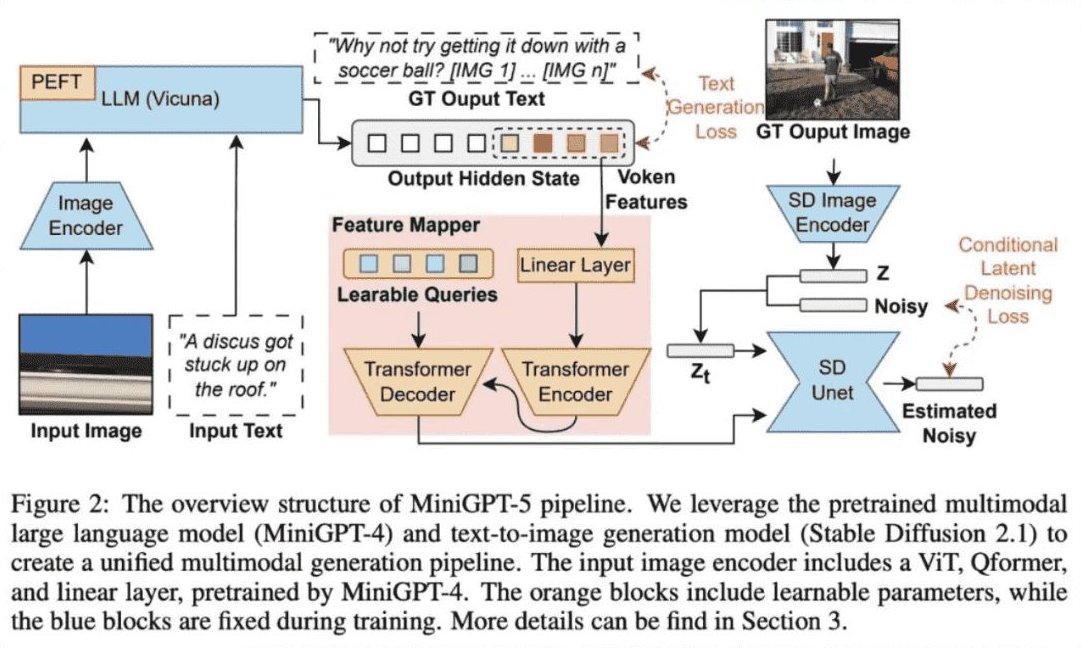
\includegraphics[width=0.98\textwidth]{images/2023-MiniGPT-5/fig-01.png}

\end{center}

% source-block: OA9Zd8XPYoO0fixhMepc4BKQnUd

\par\vspace{0.95em}\noindent{\zihao{3}\bfseries \textcolor{feishuBlue}{1.1} 多模态理解（Multimodal Understanding）模块}\par\vspace{0.28em}

% source-block: Ltexdp8pIozinVxNMD7csO4kn1d

该部分的核心是一个预训练的多模态大语言模型（论文中使用的是 MiniGPT-4 作为基础），它可以将文本 token 与输入图像编码后的视觉特征拼接在一起，得到一序列特征表示，然后进行语言理解和生成。为了让 LLM 也能在“输出”时表达图像生成信息，作者在词表中增添了“Generative Vokens”（即[IMG1]、[IMG2]…这样的可学习token），并在模型的输出层中加入对应的可学习向量，使得语言模型在生成序列时，可以自发地产生这些特殊 token，以此表征要生成的图像。\par

% source-block: JQwudJKfKoLODGxP7UVcWPaCnTe

\par\vspace{0.95em}\noindent{\zihao{3}\bfseries \textcolor{feishuBlue}{1.2} 多模态生成（Multimodal Generation）模块}\par\vspace{0.28em}

% source-block: Mzs7dBbNYou6o5xMqvIcmr7LnHg

该部分的核心是一个预训练的文本-图像扩散生成模型（Stable Diffusion 2.1）。模型需要将从 LLM 输出层得到的“voken 特征”映射到 Stable Diffusion 的条件向量空间（比如 Stable Diffusion 的 text encoder 所在的维度）。当语言模型在输出序列中生成 [IMG1] 等“voken”时，就会将这些特殊 token 的隐藏表示传递到映射模块，再通过扩散模型完成图像的生成。\par

% source-block: Ta0mdBqxjoKjUBxYYLycT0Z3npf

为了能够将 MiniGPT-4 和 Stable Diffusion 中 Unet 完美结合起来还需要对模型结构进行一定的修改：\par

% source-block: JhcTdgKk2oMUNoxYsxGcMxZMn4g

\begin{itemize}

\item 为了 LLM 的词表添加了用来表示图像的 token，称为 generative vokens\par

% source-block: VRkxdF3SxoLZCixqMbzcC5ghnsf

\item 为了将 MiniGPT-4 的输出 embedding 输入到 Unet，用一个 MLP+Transformer 进行了映射（上图中间红色框部分）\par

\end{itemize}

% source-block: HZ3id7qSGoxFtZxeoAyc4Sd8njd

\par\vspace{1.15em}\noindent{\zihao{-2}\bfseries \textcolor{feishuBlue}{2.} 模型训练}\par\vspace{0.28em}

% source-block: LB82dYkRnos9w5x6fzbcqxdXnpd

两阶段训练，Pretraining Stage和Fine-tuning Stage。\par

% source-block: KcTmdCqproM3WOxg2vlccxe9n8f

\par\vspace{0.95em}\noindent{\zihao{3}\bfseries \textcolor{feishuBlue}{2.1} Stage 1：单图-单文本 Pretraining}\par\vspace{0.28em}

% source-block: DQt2dtm4nohlSoxOpmfcXhcFnIg

第一阶段除了考虑文本生成的 loss、图像生成的 latent diffusion model loss，还要 SD 的文本编码器的输出对 generative vokens 进行了引导\par

% source-block: QzNddpU3boR9JkxQbFpcttgRnbh

使用像 CC3M 这样包含“图片+简短描述”对儿的大规模数据集。\par

% source-block: FVxOdVoqjoZxA4xugObcNUFdnKJ

训练目标：把语言模型的 voken 特征与 Stable Diffusion 的文本编码器特征对齐，从而让 MiniGPT-5 能够先学会根据“文本（caption）”来生成与描述一致的单张图像。\par

% source-block: SG2SdqhebowVDmx51NVcnOuunPe

Loss：\par\bigmath{L_{\text{Pretrain}}=\lambda_1 * L_{\text{text}}+\lambda_2 * L_{\mathrm{LDM}}+\lambda_3 * L_{\mathrm{CAP}}}

% source-block: IGSYdWuftopEvxxz63rcmwp0n7d

其中\par\bigmath{\mathcal{L}_{\text{CAP}}=\text{MSE}(\hat{h}_{\text{voken}},\,\tau_{\theta}(c))}

% source-block: ENsRdxmnKoK3eCxXvJtcx7hnnlr

\par\vspace{0.95em}\noindent{\zihao{3}\bfseries \textcolor{feishuBlue}{2.2} Stage 2：多图-多文本 Fine-tuning}\par\vspace{0.28em}

% source-block: DntpdzaN3oMK1ZxWMg3cuF4Gnkg

第二阶段使用更复杂的数据和任务来进行微调，只考虑了文本生成的 loss 和图像生成的 loss\par

% source-block: LzSBd1qcHoTlF8xihmwcHAQCnWd

数据使用的是像 VIST、MMDialog 等包含多张图与多段文本交替的复杂对话或叙事数据。\par

% source-block: V98NdhxiQoRUqvxzyimcpCxTnMc

训练目标：让模型能在长序列中，灵活地根据上下文生成文本和图像，并且能在恰当时机插入图像 [IMG] token。\par

% source-block: QujsdbVUSoR5qDxAYMOcTpGxnm4

Loss：\par\bigmath{\mathcal{L}_{\text{Fine-tune}}=\lambda_1\cdot\mathcal{L}\text{text}+\lambda_2\cdot\mathcal{L}_{\text{LDM}}}

% source-block: Qg40d2IQGoV9WlxT1rVcQX7Jngf

因为训练涉及到图像生成，所以也用了 Classifier-free Guidance 来提升条件扩散模型的性能。\par

\end{document}
